\documentclass[document.tex]{subfiles}
\begin{document}

\chapter{Algorytm Viterbiego}
\section{Opis działania i zastosowania}
\indent Alogorytm Viterbiego został stworzony i przeanalizowany przez A.J. Viterbiego w 1967r. Jego zadaniem było dekodowanie kodów splotowych. Później odkryto że posiada cechy programowania dynamicznego i wykorzystuje maksymalne prawdopodobieństwo do określenia optymalnego zestawu tranzycji pomiędzy stanami. Algorytm został oryginalnie opracowany z myślą o zastosowaniach w telekomunikacji, ale znalazł zastosowanie w innych dziedzinach, m.in. w przetwarzanie obrazów, lokalizacji i rozpoznawaniu obiektów.\cite{viterbi_tutorial}
\\
\indent Główne zastosowanie algorytmu Viterbiego polega na
dekodowaniu informacji zakodowanych przy pomocy kodów splotowych. Sekwencja kodowana $m = m_1, m_2,...,m_n$, gdzie 
$m_i$ reprezentuje pojedynczy bit informacji, a indeks oznacza kolejność przesyłania. Enkoder splotowy przekształca informację wejściową w zakodowaną sekwencję $U = G(m)$.
Wykorzystuje do tego rejestr przesuwający, sumatory modulo-2 oraz wielomiany generujące(\textit{generator polynomials}) określające związek sumatorów z rejestrem.\cite{Comm_Sklar}\cite{viterbi_tutorial}

\begin{figure}[h]
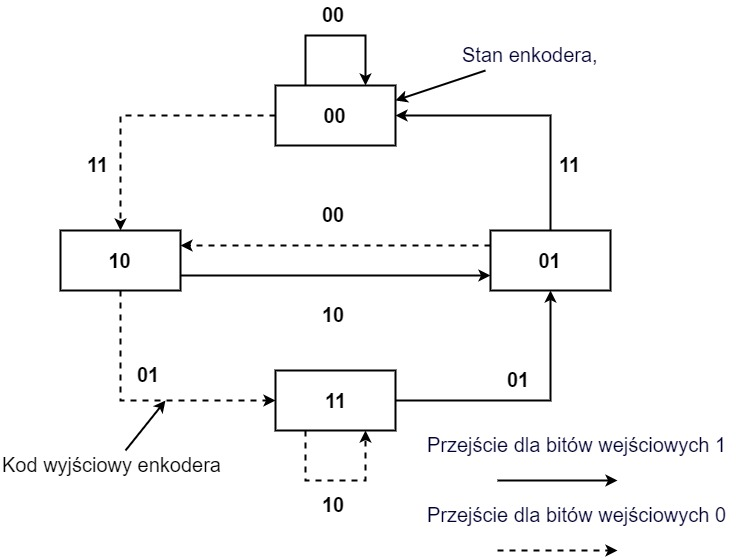
\includegraphics[scale=0.45]{conv_encoder}
\caption{Diagram stanów, dla enkodera o 3 bitowym rejestrze przesuwnym 
i dwóch sumatorach modulo-2 z wielomianami $g_1 = 111, g_2 = 101$ \protect\cite{Comm_Sklar}}
\label{fig:encoder}
\end{figure}

\clearpage
\indent Enkoder splotowy należy do klasy urządzeń zwanych automatami skończonymi(\textit{finite-state machines}), które zachowują informację o poprzednich sygnałach.
Jego działanie można zaprezentować w postaci diagramu stanów(\textit{state diagram}). Bieżący stan reprezentują pierwsze $K - 1$ bity rejestru o pojemności K, a przejścia pomiędzy stanami są określane przez kody wyjściowe.
Dla enkodera z 3 bitowym rejestrem przesuwającym i 2 bitowym wyjściem, stany są określone jako kolejno
$00, 01, 10, 11$. Diagram \ref{fig:encoder} przedstawia omawiany typ enkodera, ze wszystkimi możliwymi 
tranzycjami. Widoczne są dwa rodzaje przejść pomiędzy stanami - dla bitu wejściowego będącemu jedynką oraz dla zera. Do wizualizacji kolejnych tranzycji w czasie gdy ładowane są nowe dane do rejestru przesuwającego,
używane są diagramy kratowe(\textit{trellis diagram}).\cite{kody_splotowe}\cite{Comm_Sklar}\cite{viterbi_tutorial}
Kolumny diagramu oznaczają stany rejestru, wiersze kolejne momenty czasu $t_1, t_2, ..., t_n$. Linie łączące ze są węzły diagramu oznaczają tranzycje, które są wyzwalane pojawieniem się nowego bitu sygnału wejściowego w rejestrze enkodera(patrz rys. \ref{fig:encoder_trellis}).

\begin{figure}[h]
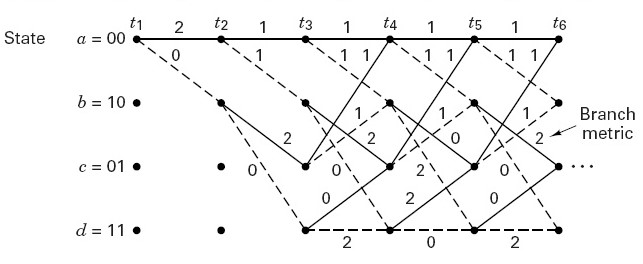
\includegraphics[scale=0.8]{encoder_trellis}
\caption{Diagram kratowy, dla enkodera o 3 bitowym rejestrze przesuwnym 
i dwóch sumatorach modulo-2 z wielomianami $g_1 = 111, g_2 = 101$ \protect\cite{Comm_Sklar}}
\label{fig:encoder_trellis}
\end{figure}

%5/31
\indent Po zakodowaniu informacji jest ona następnie poddawana modulacji - nałożenia wejściowego sygnału na analogowy sygnał nośny modulatora.\cite{Comm_Sklar}\cite{modulacja_put} Sygnał cyfrowy ze względu na małą częstotliwość jest podatny na zakłócenia w trakcie transferu. Stosując modulację 
sygnałem analogowym o wyższej częstotliwości możliwe jest przesyłanie informacji na większe odległości oraz zmniejszenie wpływu zakłóceń.
Sygnałem nośnym najczęściej są sygnały sinusoidalne, np. w postaci\cite{modulacja_agh_amp}\cite{modulacja_put}:

\begin{equation}
    f_c(t) = A_c cos(\omega t + \theta)
\end{equation}
\label{eq:module_carrier}
\myequations{Funkcja sygnału nośnego modulatora\cite{modulacja_agh_amp}}

Na podstawie równania \ref{eq:module_carrier} można stwierdzić że występują trzy parametry, na które można wpłynąć do modyfikacji modulowanego sygnału - amplituda $A_c$, częstotliwość $\omega$ oraz faza $\theta$. Dlatego wyróżniamy trzy rodzaje modulacji(patrz rys.\ref{fig:modulation}):
\begin{itemize}
    \item modulacja częstotliwości - jest osiągana poprzez zmianę częstotliwości sygnału w zależności, czy w danym momencie występuje zmiana z 0 na 1(zwiększenie częstotliwości), czy z 1 na 0(zmniejszenie częstotliwości).
    \item modulacja amplitudy - polega na zmodyfikowaniu amplitudy sygnału nośnego przez amplitudę sygnału zakodowanego.
    \item modulacja fazy - różnica pomiędzy 0 i 1 w sygnale wejściowym jest reprezentowana przez zmianę startu sygnału sinusoidalnego nośnika, np. 0\degree dla 0 i 180\degree dla 1.
\end{itemize}
\clearpage
\begin{figure}[h]
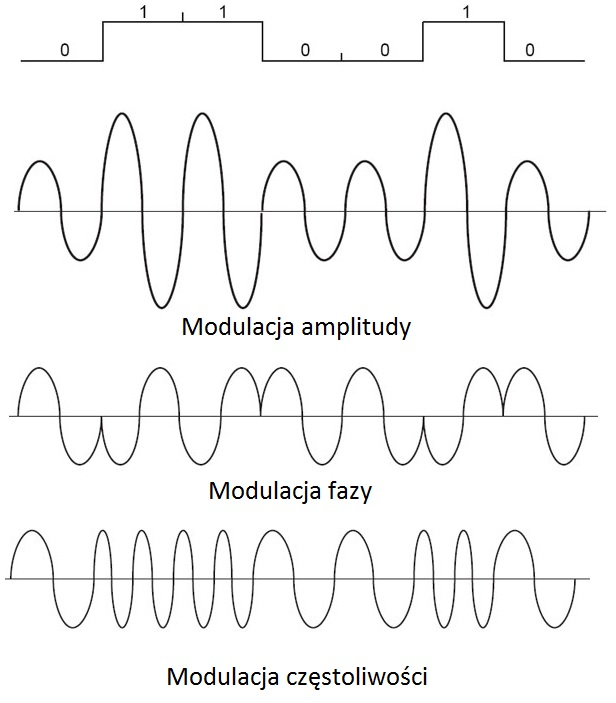
\includegraphics[scale=0.55]{modulation}
\caption{Rodzaje modulacji sygnału cyfrowego \protect\cite{Comm_Sklar}\cite{modulacja_put}}
\label{fig:modulation}
\end{figure} 

\indent Odbiornik dostaje zakodowaną, modulowaną i zakłóconą informację. W pierwszej fazie odczytywania przesłanego sygnału niezbędna jest jego demodulacja. Polega ona na odzyskaniu sygnału z wyjścia enkodera przed modulacją.
Dla sygnału modulowanego amplitudowo \textbf{AM} demodulacja może być przeprowadzona poprzez użycie detektora diodowego oraz filtracji niepożądanych wysokich częstotliwości.\cite{demodulation_am}
W przypadku demodulacji częstotliwościowej \textbf{FM} i fazy \textbf{PM}, wykorzystywane są detektory \textbf{PLL}(\textit{Phase Locked Loop} - pętla synchronizacji fazy)\cite{demodulation_fmpm}.

\indent W celu odczytania informacji zakodowanej enkoderem splotowym stosowany jest dekoder
wykorzystujący algorytm Viterbiego. Wykorzystuje on strukturę diagramu kratowego do obliczenia optymalnej
kombinacji przejścia pomiędzy jego stanami. Do określenia najlepszego wariantu przejścia ze stanu $i$ do stanu $i+1$ wybierana jest tranzycja o najmniejszej odległości Hamminga\cite{Comm_Sklar} względem fragmentu kodu po demodulacji. Jeśli występuje kilka możliwych przejść do danego stanu, wybierane jest te, które ma największe prawdopodobieństwo - najmniejszą odległość Hamminga, a reszta jest odrzucana.

%wrzucic trellis z dystansami hamminga oraz z kodem enkodera, dekodera, oraz wejściem enkodera do porównania



%indent
%opisać rozpatrywany przypadek wykorzystania viterbiego
%do wyznaczania linii - arytkuły mazurek

%i chyba styka
\clearpage
\section{Implementacja w języku C++}
\indent Tworząc aplikację wykorzystującą algorytm Viterbiego do lokalizacji linii
na obrazie cyfrowym skorzystano z nowych funkcjonalności standardu C++11. 
Zdjęcia na, których szukano linii były wczytywane używając funkcji biblioteki
CImg. Reprezentowane przez obiekty \code{Cimg<T>}, dane pikseli zdjęcia były kopiowane do
dynamicznie zaalokowanych tablic jednowymiarowych obiektu \code{unique\_ptr}. Skorzystano z obiektu \code{unique\_ptr} w celu przechowywania wskaźnika do dynamicznie zaalokowanej pamięci, ze względu na funkcję automatycznego zwalniania zaalokowanych zasobów po wywołaniu destruktora \code{unique\_ptr}.  

%opis listinigu opencl_viterbi.cpp
\subsection{Wersja szeregowa}

%listing z viterbiLineDetect - nie pokazywac całego
\lstinputlisting[language={C++}, label={lst:viterbi_serial}, caption=Szeregowa implementacja algorytmu Viterbiego do wykrywania linii, linerange=224-297, firstnumber=224]{viterbi_source/Viterbi.cpp} 

%fragment inicjalizacja
\lstinputlisting[language={C++}, label={lst:viterbi_serial}, caption=Szeregowa implementacja algorytmu Viterbiego do wykrywania linii, linerange=224-240, firstnumber=224]{viterbi_source/Viterbi.cpp} 


%opisać wszystkie fragmenty z odniesieniem do schematu ogólnego algorytmu - shcemat z atykułów i wzory
\subsection{Wersja równoległa - C++11}
To jest podrozdział 2 rozdziału 2
\subsection{Wersja równoległa - OpenCL}
To jest podrozdział 3 rozdziału 2
\end{document}